\documentclass[tikz]{standalone}
\usetikzlibrary{calc,patterns,angles,quotes}
\usepackage{pgfplots}
\pgfplotsset{compat=newest}

\pagestyle{empty}

\begin{document}
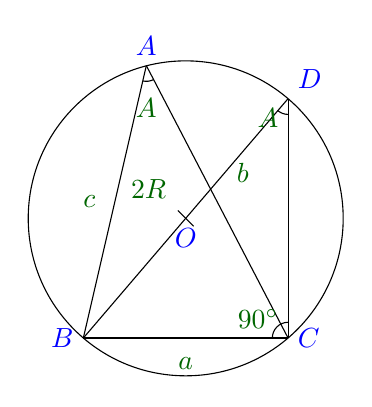
\begin{tikzpicture}
  \draw (0,0) circle (2cm);
  \coordinate [label={[blue]below:$O$}] (O) at (0,0);
  \draw (0.1, -0.1) -- (-0.1, 0.1);
  \coordinate [label={[blue]above:$A$}] (A) at (-.5, 1.94);
  \coordinate [label={[blue]above right:$D$}] (D) at (1.3, 1.52);
  \coordinate [label={[blue]right:$C$}] (C) at (1.3, -1.52);
  \coordinate [label={[blue]left:$B$}] (B) at (-1.3, -1.52);
  \draw (B) -- (C);
  \draw (A) -- (B);
  \draw (B) -- (D);
  \draw (C) -- (A);
  \draw (C) -- (D);
  \node[label={[black!60!green]left:$c$}] at ( $ (A)!0.5!(B) $ ) () {};
  \node[label={[black!60!green]below:$a$}] at ( $ (C)!0.5!(B) $ ) () {};
  \node[label={[black!60!green]above right:$b$}] at ( $ (C)!0.5!(A) $ ) () {};
  \node[label={[black!60!green]above left:$2R$}] at ( $ (B)!0.5!(D) $ ) () {};
  \draw pic [draw, angle radius=0.2cm] {angle=B--A--C};
  \coordinate [label={[label distance=0.3cm, black!60!green]below:$A$}] (A1) at (-.5, 1.94);
  \draw pic [draw, angle radius=0.2cm] {angle=B--D--C};
  \coordinate [label={[black!60!green]below left:$A$}] (D1) at (1.3, 1.52);
  \draw pic [draw, angle radius=0.2cm] {angle=D--C--B};
  \coordinate [label={[black!60!green]above left:$90^\circ$}] (C) at (1.3, -1.52);
\end{tikzpicture}
\end{document}
